\documentclass[border=10pt]{standalone}

\usepackage{tikz}
\usepackage{tikzsymbols}
\usetikzlibrary{calc,patterns,shapes.geometric}

\def\centerarc[#1](#2)(#3:#4:#5){\draw[#1] ($(#2)+({#5*cos(#3)},{#5*sin(#3)})$) arc (#3:#4:#5);}

\begin{document}
	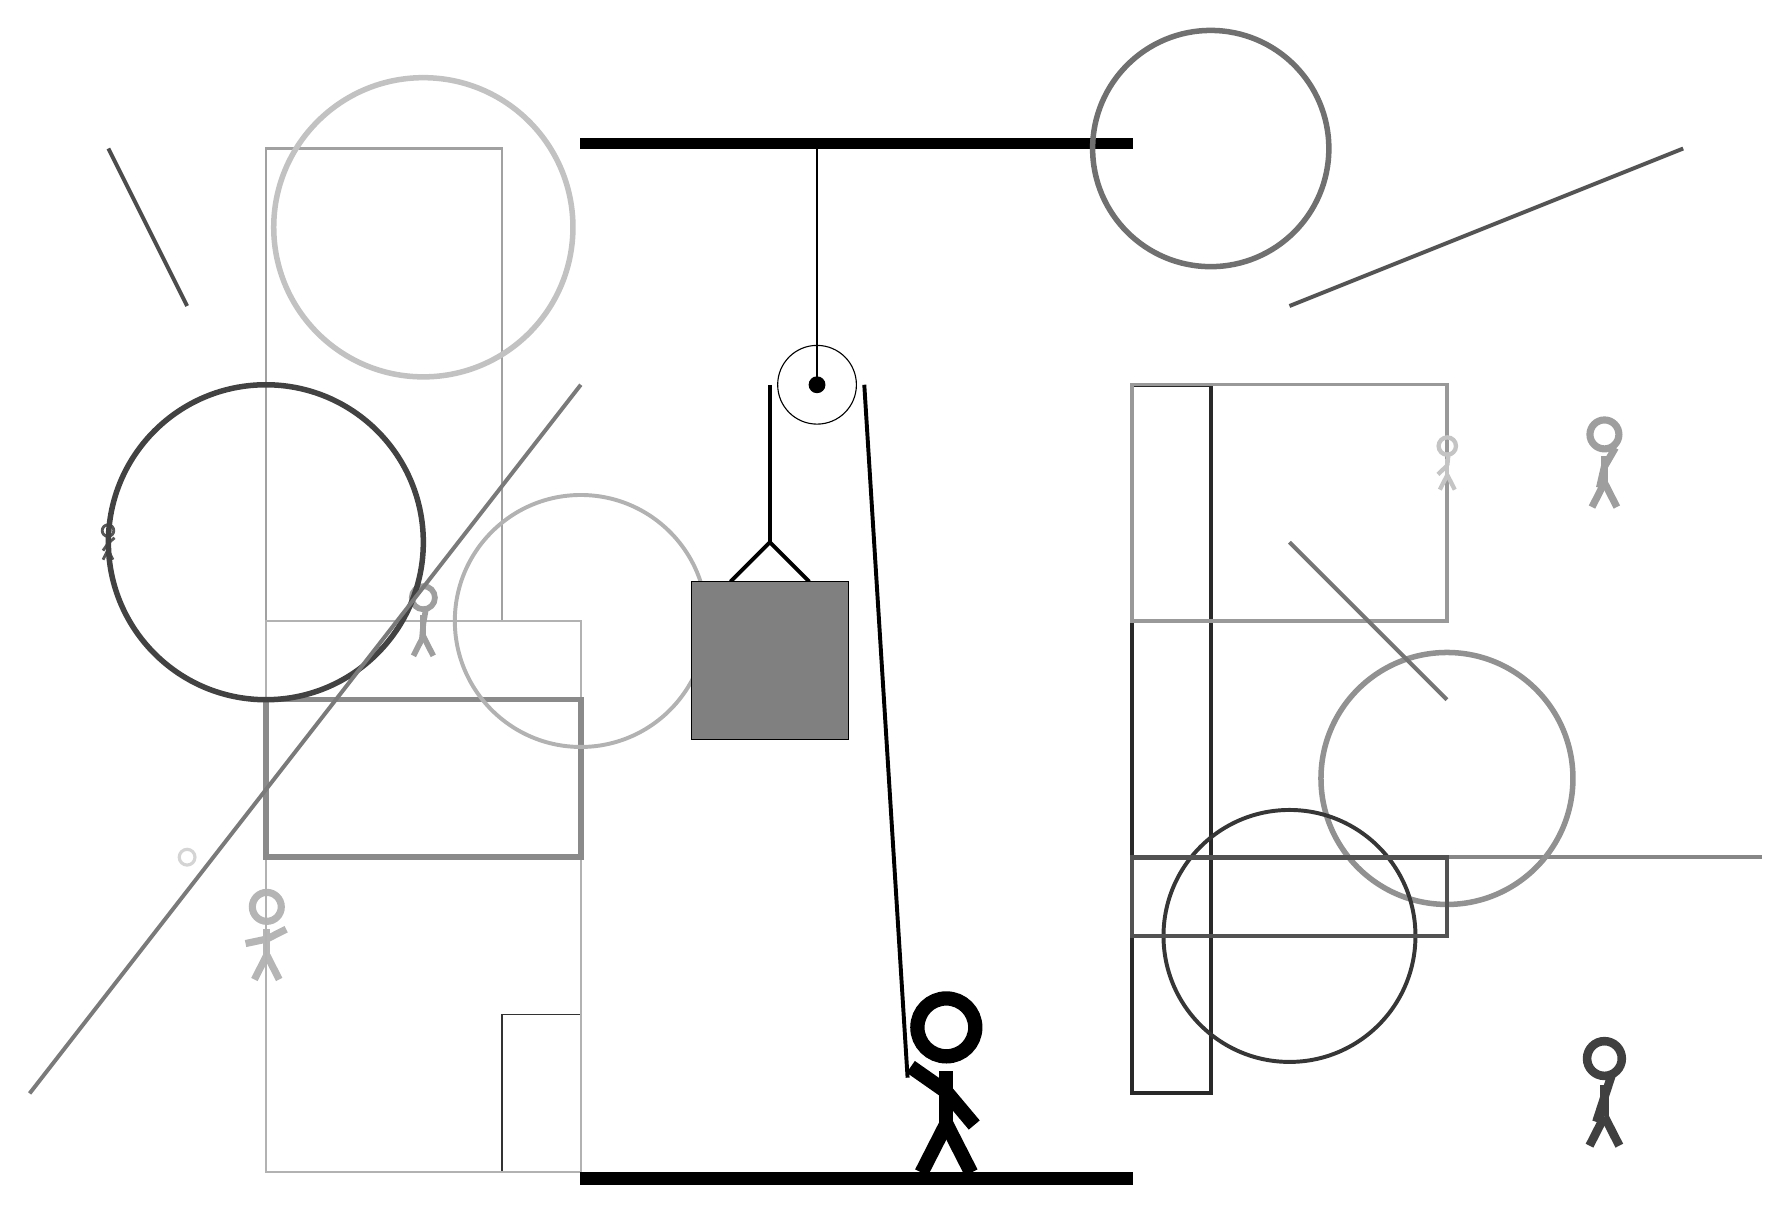
\begin{tikzpicture}
		%%%%% START %%%%%
		
		\draw[fill=black] (-2, 10) rectangle (5, 10.125);
		
		\draw (1, 7) circle (0.5);
		\draw[fill=black] (1, 7) circle (0.1);
		\draw (1, 10) -- (1, 7);
		
		\draw[line width=0.5mm, color=black!47](7, 1) -- (13, 1);
		
		\node[line width=0.2mm, color=black!29] at (-6, 0) {\Strichmaxerl[5][12][27]};
		\draw [line width=0.4mm, color=black!17](-7, 1) circle (0.1);
		\node[line width=0.2mm, color=black!75] at (11, -2) {\Strichmaxerl[6][72][72]};
		\draw[line width=0.5mm, color=black!84] (5, 7) rectangle (6, -2);
		\draw[line width=0.3mm, color=black!37] (-3, 10) rectangle (-6, 4);
		\draw[line width=0.2mm, color=black!80] (-3, -1) rectangle (-2, -3);
		\draw[line width=0.2mm, color=black!30] (-2, 4) rectangle (-6, -3);
		\draw [line width=0.7mm, color=black!24](-4, 9) circle (1.9);
		\draw[line width=0.4mm, color=black!40] (5, 4) rectangle (9, 7);
		\node[line width=0.6mm, color=black!66] at (-8, 5) {\Strichmaxerl[2][55][41]};
		
		\draw [line width=0.7mm, color=black!43](9, 2) circle (1.6);
		\draw[line width=0.5mm, color=black!70](-7, 8) -- (-8, 10);
		\draw[line width=0.5mm, color=black!54](7, 5) -- (9, 3);
		\draw [line width=0.5mm, color=black!79](7, 0) circle (1.6);
		\node[line width=0.3mm, color=black!38] at (-4, 4) {\Strichmaxerl[4][85][80]};
		
		\draw[line width=0.7mm, color=black!46] (-2, 1) rectangle (-6, 3);
		\draw [line width=0.7mm, color=black!56](6, 10) circle (1.5);
		\node[line width=0.6mm, color=black!23] at (9, 6) {\Strichmaxerl[3][44][84]};
		\draw [line width=0.7mm, color=black!74](-6, 5) circle (2.0);
		\node[line width=0.5mm, color=black!38] at (11, 6) {\Strichmaxerl[5][77][60]};
		\draw[line width=0.6mm, color=black!68] (5, 0) rectangle (9, 1);
		
		\draw[line width=0.5mm, color=black!67](7, 8) -- (12, 10);
		\draw [line width=0.5mm, color=black!30](-2, 4) circle (1.6);
		\draw[line width=0.5mm, color=black!52](-2, 7) -- (-9, -2);
		
		
		\draw[line width=0.5mm] (-0.1, 4.5) -- (0.4, 5.0) -- (0.9, 4.5);
		\draw[fill=black!50] (-0.6, 4.5) rectangle (1.4, 2.5);
		
		\draw[line width=0.5mm] (0.4, 7) -- (0.4, 5.0);
		\centerarc[line width=0.5mm](1, 7)(0:180:0.6);
		\draw[line width=0.5mm](1.6, 7) -- (2.15, -1.8);
		
		\node at (2.6, -1.9) {\Strichmaxerl[10][-35][-50]};
		
		\draw[fill=black] (-2, -3) rectangle (5, -3.15);
		
		%%%%% END %%%%%
	\end{tikzpicture}
\end{document}